\section{Hardware Components}

New instrumentation modules have been designed by JLab that take advantage of the higher performance and elegant back-plane connectivity of the VITA 41 standard or ``VXS'', defined as VME with serial extensions. 
VXS was selected as the 12~GeV data acquisition back-plane foundation for the front-end detector readout and trigger hardware interface because this standard offered a method to easily synchronize and pass signals between each of the payload slots to a central switch fabric slot. At JLab a dual star back-plane configuration is used, and one switch slot is used for the trigger processing and one switch slot is used to distribute the essential timing and synchronization signals to each of the front-end boards.

The trigger processor switch slot board manages the high-speed gigabit signaling from each of the payload slots, where eight differential pairs connect from the payload slots to the switch slots. The VXS crates are manufactured by WIENER and the back-plane can support up to 8~Gb/s. The payload boards use Xilinx Virtex V technology, and these FPGAs have up to 6.25~Gbps transceivers. The payload boards are designed to run these high-speed gigabit transceivers at a maximum of 5~Gpbs to transfer trigger data to the trigger processor module. 

The design challenges for reliable and successful transmission of gigabit serial data over the VXS backplane requires the investment of high-speed circuit board layout and routing tools.  The FPGA selection requirements include at least four full duplex gigabit transceivers, user I/O pin count $>$~500, and fast integrated block memory with multi-rate FIFO logic. We use circuit board routing simulation tools such as Mentor Graphics HyperLynx [\ref], which are invaluable for critical simulation and verification of circuit board signal integrity for the gigabit transmission paths before the manufacturing process.  The FPGA devices that we use are capable of 6.25~Gb/s serial transfer, and we have designed our circuit boards with signal integrity techniques using standard FR4 circuit board material to achieve $>$~2.5~Gb/s, which meets the data transfer bandwidth requirements. 
Another significant investment required for the hardware verification of the gigabit transceivers was a digital signal analyzer with 8~GHz bandwidth to measure and record the backplane and fiber optic gigabit transceiver performance and to perform jitter analysis on the critical system clock and synchronization signals with at least 1~ps resolution.  We used the Tektronix jitter analysis software which is a critical tool for the verification of our system clock, and for measurements of the phase controlled jitter attenuated clock provided by the Signal Distribution (SD) switch card in every crate. The investment of firmware development tools from FPGA industry leaders Xilinx and Altera were also taken into consideration for the upgrade path to VXS. We use the Xilinx Aurora protocol for serial transmission as it is robust and simple, and is included with the FPGA development tools.  


\subsection{Fiber Optic Trigger distribution system}

As shown in Fig.~\ref{fig:hardwarediagram}, the digital sum value from each VTP in the front-end crate, and the distribution of the global clock, synchronization, and trigger commands from the global trigger hardware, use a separate fiber optic cable.  The crate sum fiber link is shown in orange, and the critical timing signals distributed to each front-end crate are blue.  Each fiber optic link makes use of the Avago POP4 fiber optic transceivers and parallel OM3-rated glass fiber cable with MTP connections. These fiber optic transceivers operate at 3.125 Gb/s for an aggregate bandwidth of 10 Gb/s which is ample enough for the summing information that is sent forward to the global trigger processing hardware.  The fiber link used for the distribution of the global clock, critical timing signals, and trigger commands runs at 1.25~Gb/s.

\begin{figure}[hbt]
	\centering
	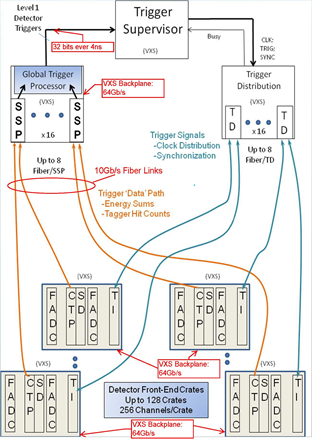
\includegraphics[width=1.0\columnwidth,keepaspectratio]{img/hardware_diagram.png}
	\caption{Hardware diagram with the implemented fiber links scheme.}
	\label{fig:hardwarediagram}
\end{figure}


\subsection{VXS/VME crates}

Previous experiments with the original CLAS spectrometer (\ref) used the VXI standard, which was a new extension of the original VME standard. VXI offered a method to distribute clock and other timing signals with low skews via the back-plane. 9U circuit boards were used that offered a large number of front panel input/output connections to handle the six sectors of the CLAS detectors that contributed to the level 1 trigger. The detector signals were acquired with FastBus ADC and TDC or in some instances, from VME or even CAMAC modules. 

During the initial design phase of the 12~GeV experiments the requirements of a 200~KHz sustained trigger rate demanded that the front-end modules adopt a new method of handling precision timing and synchronization over dozens of front-end crates. The latest technology at the 12~GeV inception included FPGA devices with high-speed serial transceivers built into the silicon fabric. A new VME extension was also emerging at the same time, which was labeled VXS, and defined a new high-speed gigabit connector with links between the VME slots and eight serial links to common switch slots. The VXS standard was declared as VITA 41 and several new standards have emerged in the past decade that expand the use of gigabit serial transmission via the crate back-plane. For the 12~GeV experiment era, we now have thousands of custom VXS payload and switch slot modules and hundreds of VXS front-end crates. Complex experiments and high channel count detectors make use of these custom VXS boards  designs for all four experimental halls at JLab.

\subsection{VME Crate Controllers}

The high-speed data physics acquistion and trigger systems for the JLab 12~GeV experiments have been standardized on the VME64X and VXS backplane and crate enclosure form-factor. In addition to the custom electronics that reside in these crates, there must also be a single ``controller'' for each crate. Considering all four experimental halls, this exceeds 100 controllers.

There are many commercial off-the-shelf options for this type of controller, and our general requirements do not extend beyond what is currently commercially available. We do have some specific requirements that narrowed the viable choices.

We purchased VME controllers from several vendors for development purposes and made a significant investment in custom software that runs on all of the existing boards. We also benchmarked our code and have come to expect certain ``minimum'' requirements for performance from the chosen architecture within an specified Linux operating system.

We also expect a certain minimum 10 year timeframe in which these controllers will be supported by the vendor with respect to the avilable parts, repair, and software updates. VME controller requirements are summerized in following list:

\begin{itemize}
	\item Single slot VME form-factor - no required rear transition module
	\item Intel Core i7 dual or quad core embedded processer 2~GHz (or greater)
	\item Hyperthreading and 64~bit arch support
	\item 4 GBytes DDR3 (1066~MHz) ECC SDRAM (or greater)
	\item Front panel gigabit ethernet and serial port console
	\item 1 x4 PCI Express XMC expansion slot (or greater)
	\item VME320-interface using the Tundra Tsi148 chip
	\item support for all VME transfer modes including 2eSST
	\item VXS optional: interface supporting both VITA 41.3 (Gig E) and 41.4 (PCIe) standards.
\end{itemize}

After several different boards were evaluated we purchased XVR16 Intel forth Generation 4-core i7-based rugged VME single board computers from GE (see Fig.~\ref{fig:XVR16diagram}). They were installed in the 70+ crates for CLAS12 and have demonstrated excellent performance and reliability. Most of the controllers send data over their built-in 1~GBit link, while for few of them, a 10~GBit daughter board was installed to increase the bandwidth. The maximum data rate from a single crate in CLAS12 never exceeds 130~MB/s, and with that rate 4-core controllers are able to handle the VME data polling, data processing, and sending data over the network without any issues. 

\begin{figure}[hbt]
	\centering
	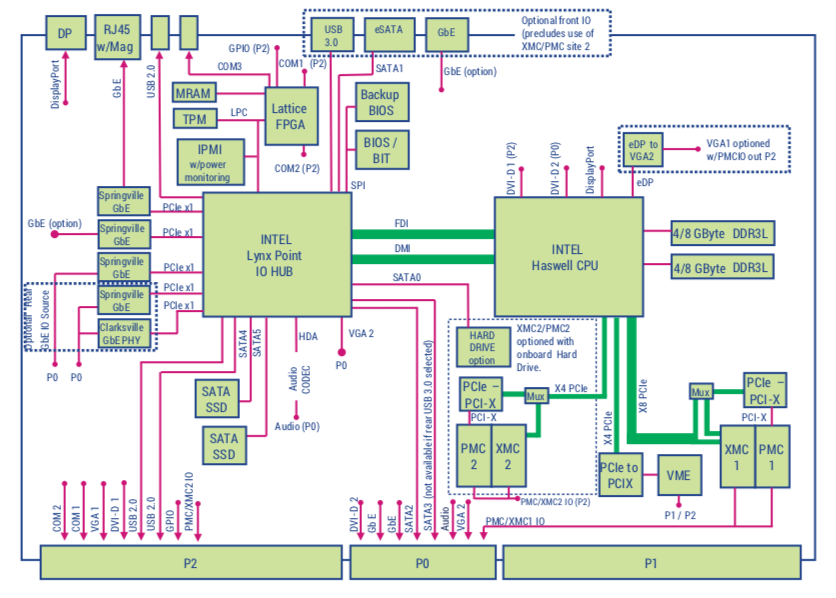
\includegraphics[width=1.0\columnwidth,keepaspectratio]{img/XVR16_diagram.png}
	\caption{Block diagram of the XVR16 VME crate controller}
	\label{fig:XVR16diagram}
\end{figure}



\subsection{Trigger Distribution System Modules (TS, TD, TI)}
	
The TCS (TRIGGER, CLOCK, SYNC, and BUSY) distribution system [\ref] is the hardware interface to bridge the trigger and the DAQ.  The TCS system receives the trigger decision from the trigger system, and initiates data readout for the DAQ system by distributing the readout trigger (TRIGGER) signal.  Additionally, it distributes a 250~MHz system clock (CLOCK) to pipeline the system, and it distributes an encoded synchronous signal (SYNC) for the system synchronization.  It monitors the frontend electronics’ status (BUSY) and makes sure of the smooth data readout of the experiments. Fig.~\ref{fig:TCSdiagram} shows a diagram of the trigger and TCS distribution.

\begin{figure}[hbt]
	\centering
	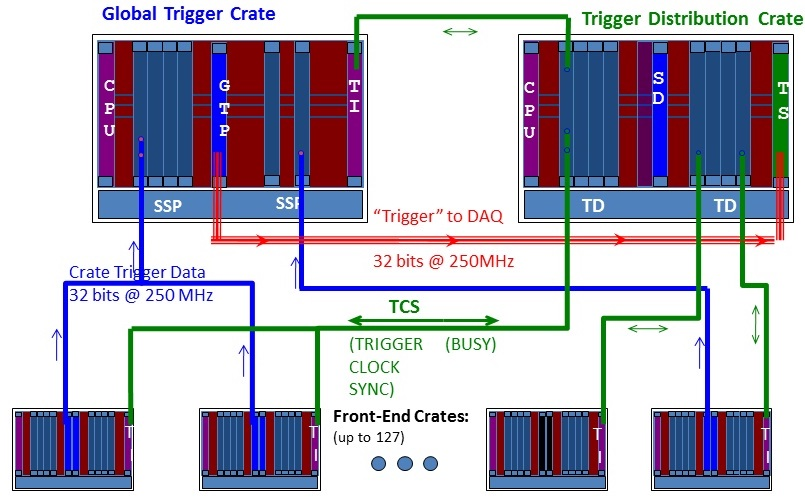
\includegraphics[width=1.0\columnwidth,keepaspectratio]{img/TCSdiagram.jpg}
	\caption{Diagram of the trigger and TCS distribution}
	\label{fig:TCSdiagram}
\end{figure}


The main hardware of TCS distribution system includes a Trigger Supervisor (TS)[2] board (Fig.~\ref{fig:TSused}, Fig.~\ref{fig:TSdiagram}), Signal Distribution (SD) boards, Trigger Distribution (TD)[3] boards  (Fig.~\ref{fig:TDused}), Trigger Interface (TI)[3] boards  (Fig.~\ref{fig:TIused}, Fig.~\ref{fig:TIdiagram}), VXS crates, and optic fibres.  The TS board, one SD board, and up to sixteen TD boards are located in the global TCS distribution VXS crate.  One TI board and one SD board and/or one FANIO board are located in each frontend crate.  The electronics boards are custom designed and produced for the 12 GeV upgrade.  Field Programmable Gate Arrays (FPGA) are used for TCS generation, control and decoding.  Optical Fibres and high-speed differential backplane connections are used to transmit signals at high speed and long distance.  

\begin{figure}[hbt]
	\centering
	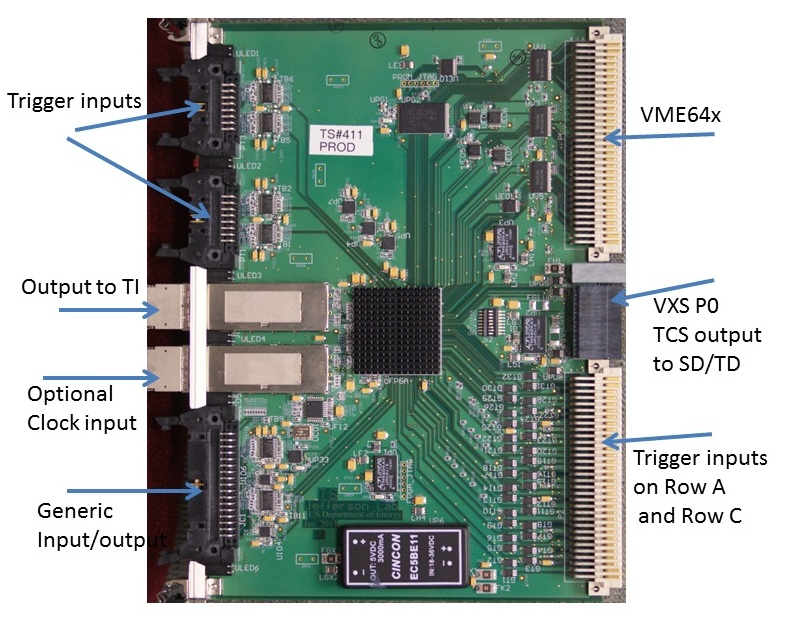
\includegraphics[width=1.0\columnwidth,keepaspectratio]{img/TSused.jpg}
	\caption{TS board}
	\label{fig:TSused}
\end{figure}

\begin{figure}[hbt]
	\centering
	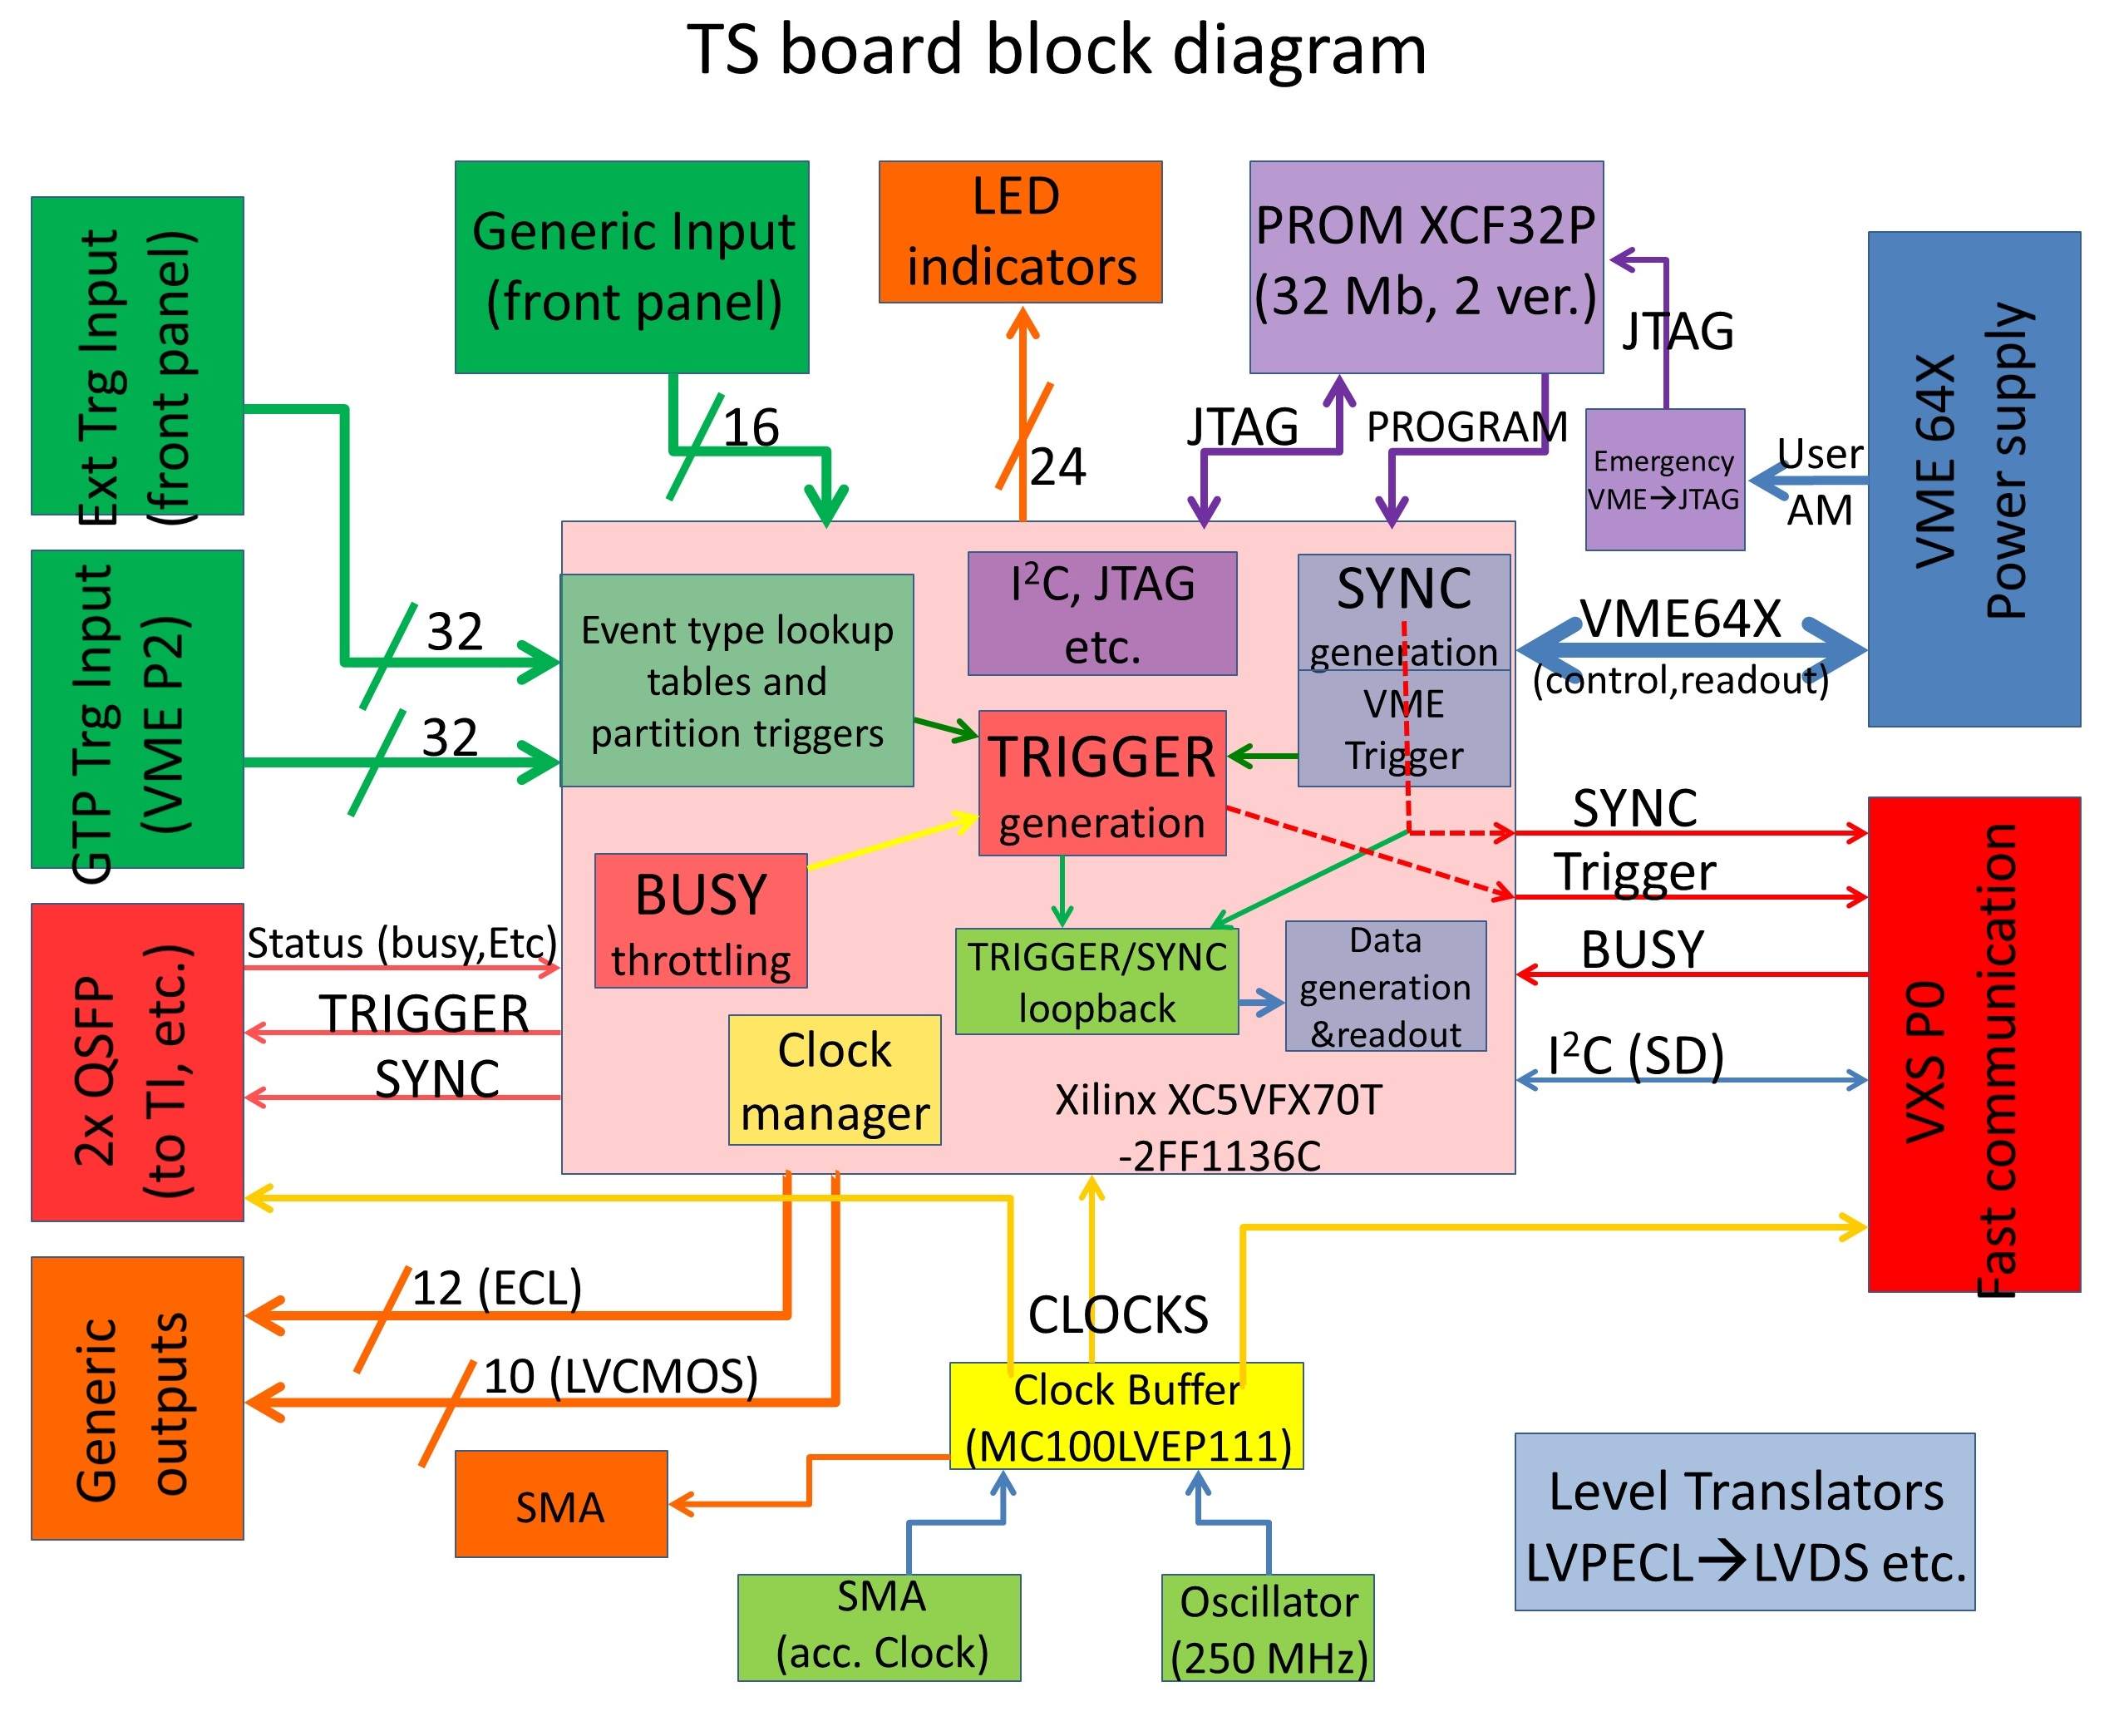
\includegraphics[width=1.0\columnwidth,keepaspectratio]{img/TSdiagram.jpg}
	\caption{TS board diagram}
	\label{fig:TSdiagram}
\end{figure}

\begin{figure}[hbt]
	\centering
	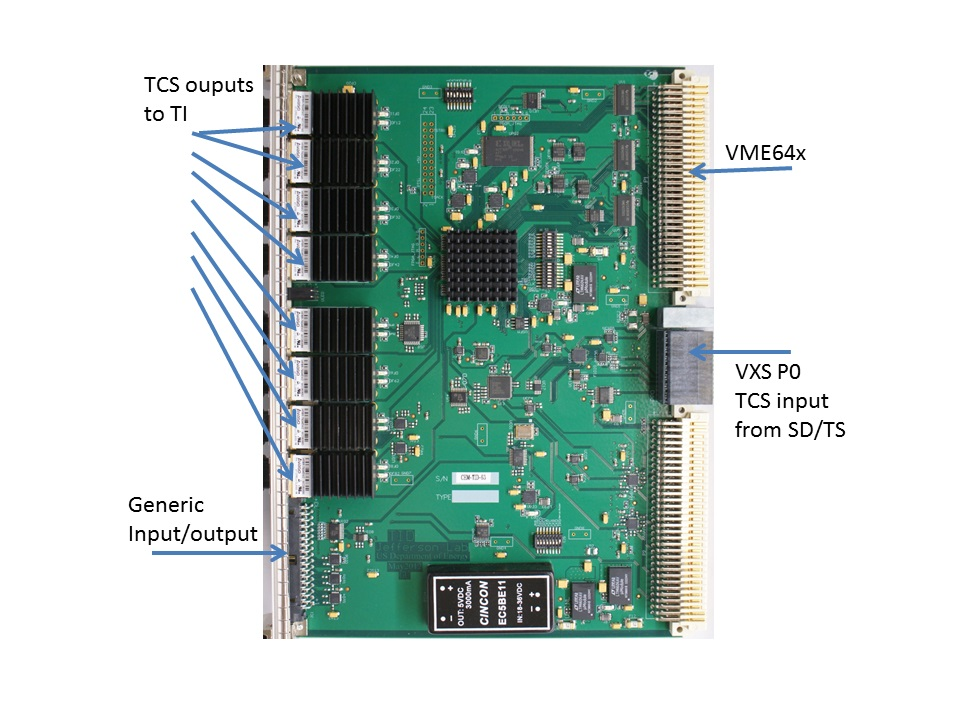
\includegraphics[width=1.0\columnwidth,keepaspectratio]{img/TDused.jpg}
	\caption{TD board}
	\label{fig:TDused}
\end{figure}

\begin{figure}[hbt]
	\centering
	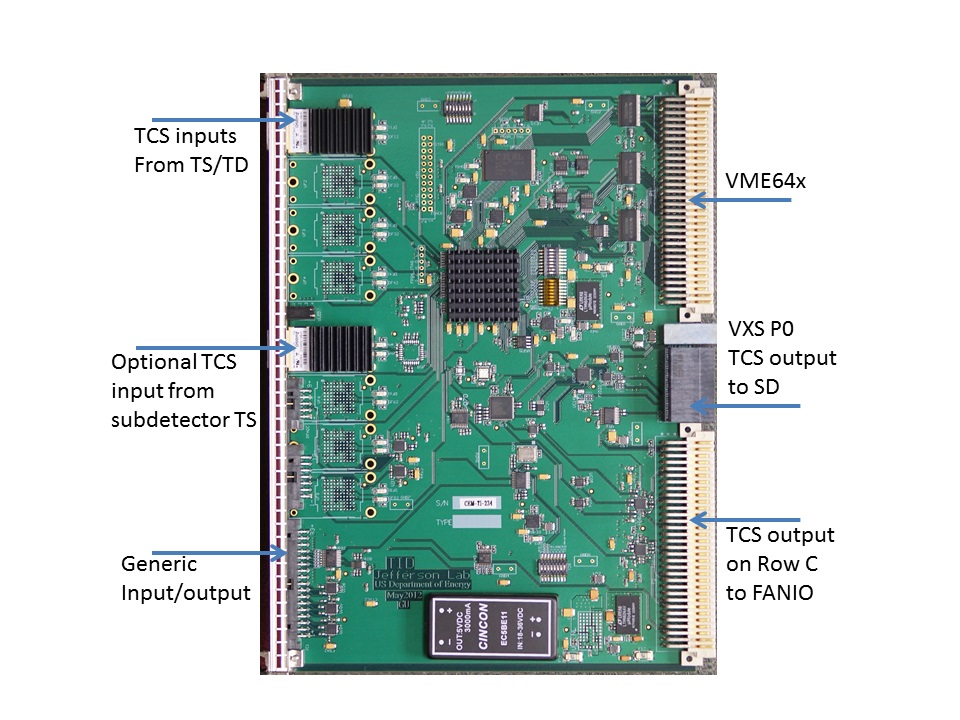
\includegraphics[width=1.0\columnwidth,keepaspectratio]{img/TIused.jpg}
	\caption{TI board}
	\label{fig:TIused}
\end{figure}

\begin{figure}[hbt]
	\centering
	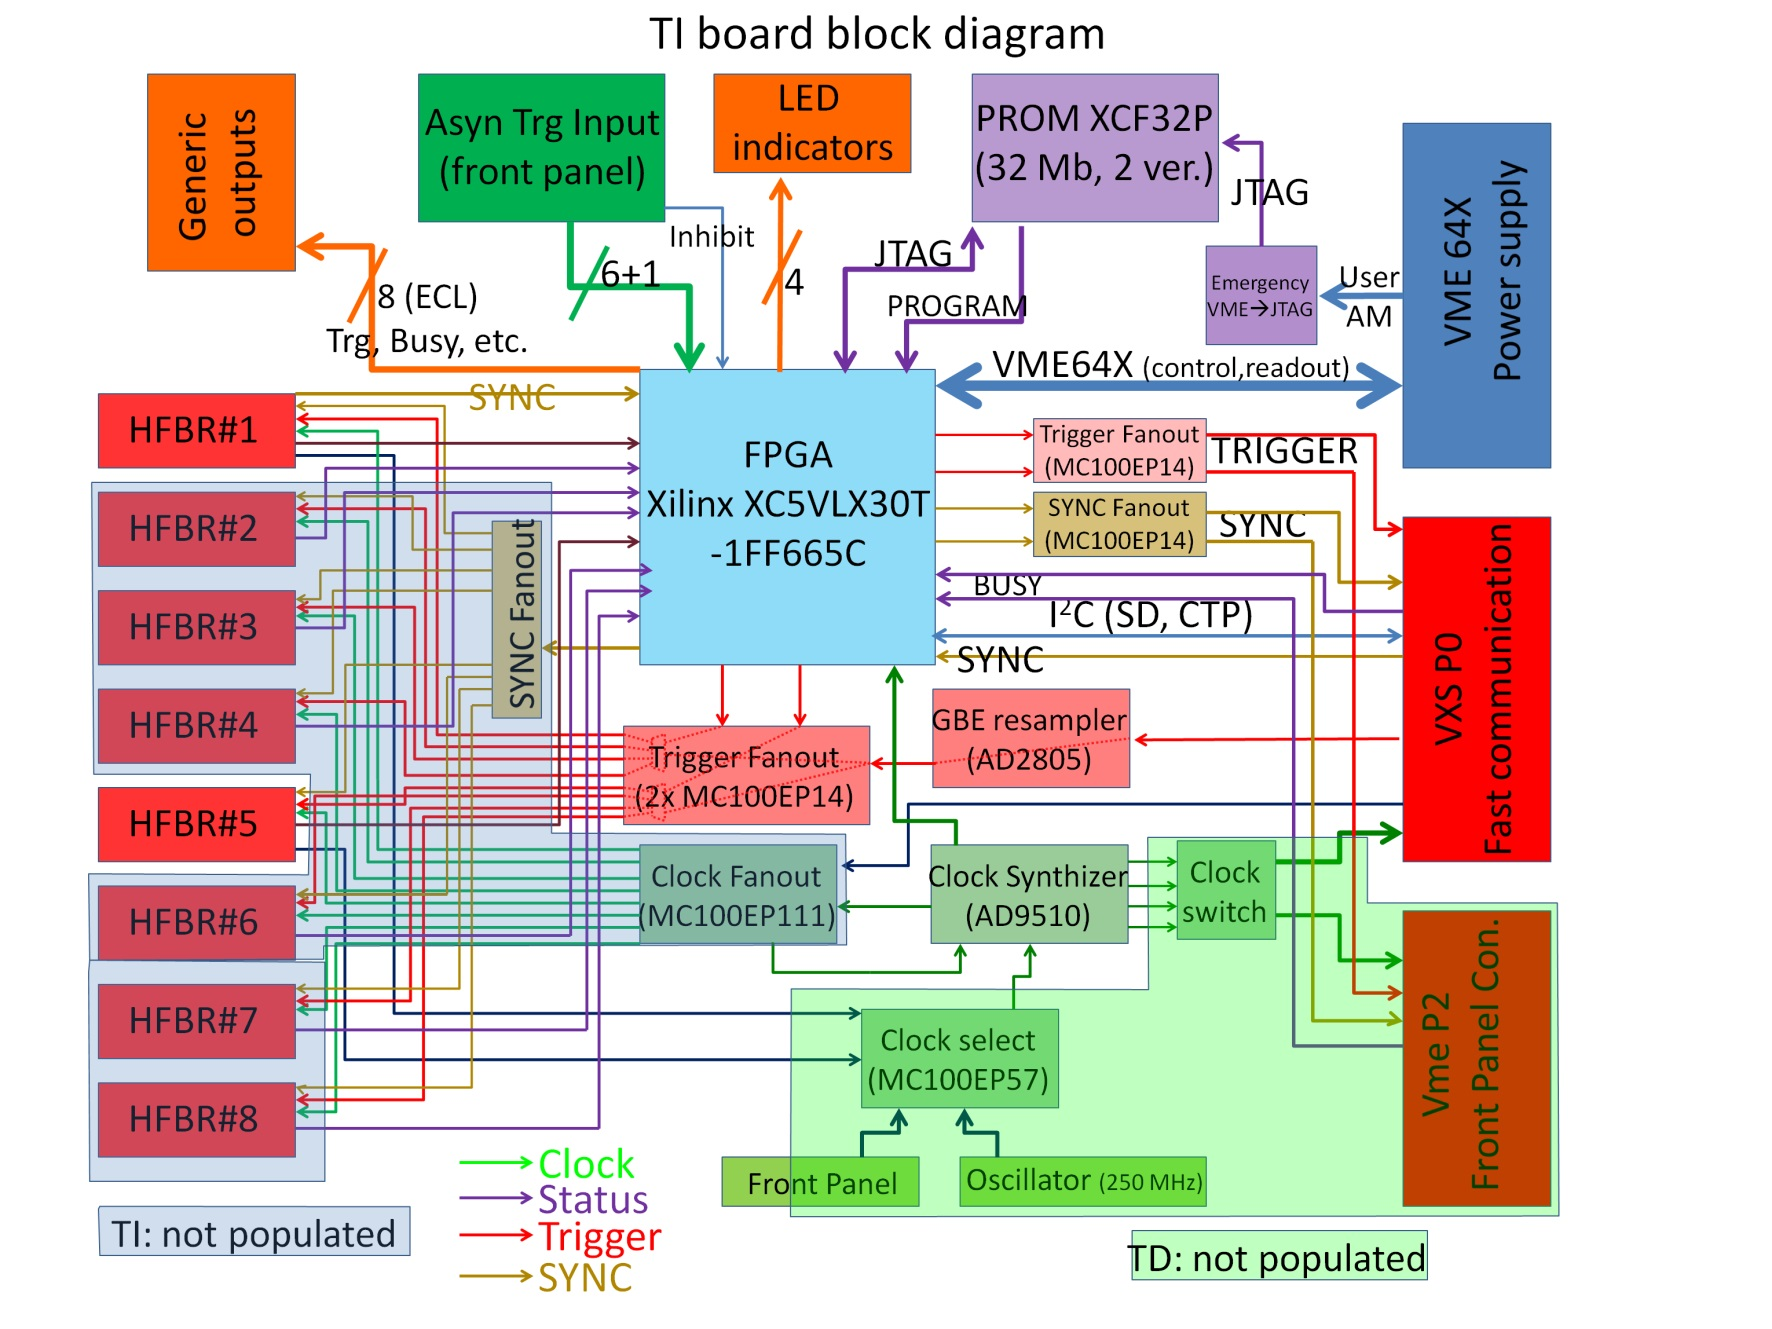
\includegraphics[width=1.0\columnwidth,keepaspectratio]{img/TIdiagram.jpg}
	\caption{TI board diagram}
	\label{fig:TIdiagram}
\end{figure}


A.	Clock distribution

The TCS system uses the same 250 MHz clock, which comes from the TS in the global trigger distribution crate.  This clock is either generated by TS’ on board oscillator or its front panel input.  The clock is fanned out to the VXS P0 connector, then to the SD board.  The SD fans out the clock to TD boards via VXS P0 backplane.  The TD boards further fan out to the TI boards via optic fibres.  The TI uses this clock to generate clocks with proper frequencies (250 MHz, 125 MHz, 62.5 MHz, 31.25 MHz and 41.67 MHz) and sends the clocks to the front end crate SD board, and the SD fans out to the front-end DAQ modules (TDC, ADC).  The fan-out buffer level is minimized on every board to limit the clock jitter.  The slower clocks derived from system clock are phase aligned thanks to the Analog Devices AD9510 with a synchronous phase re-alignment command.  The clock jitter is about one ps measured at the frontend electronics.  The clock distribution skew can be adjusted by the SD clock delay if necessary.

B.	SYNC distribution

The TS generates and distributes the SYNC signal.  The SYNC is an encoded four bits serialized command transferred at 250 Mbps synchronized with the system clock.  Normally, the serial SYNC line stays at logic high (or ‘1’).  When transferring a SYNC command, the SYNC goes to logic low for one bit, followed by the 4-bit command code.  After the 4-bit SYNC command, the SYNC goes to logic high again.  There is a minimum of four ‘1’s before the next cycle begins.  The SYNC start is phase aligned to the 62.5 MHz clock used for the trigger word transfer, the 41.67 MHz clock used for CAEN TDC boards, and the 31.25 MHz clock used for Flash TDC boards.  This phase relation is used to synchronize the slower clocks on the TI to the 62.5 MHz clock on TS.  This also limits the SYNC command to no more than one per 96 ns.  To facilitate the AC coupled optical transceivers, the SYNC is Manchester encoded on the TS and the TD, and Manchester decoded on the TI and the TD.
The SYNC is phase aligned with the 250 MHz system clock on TI boards using their FPGA’s IODELAY.  The SYNC is synchronized across the TI boards by applying different delays on the individual TI boards.  The delays are determined by the fibre latency measurement.  
The spare fibres between TD and TI boards are used to measure the fibre latency.  The TI sends a test signal to the TD through one fibre, and the TD loops back the signal through another fibre.  The TI measures the delay between the test pulse and the looped back test pulse using the FPGA counter and the carry chain in FPGA.  As the fibre skew is small (less than 1 ns for 100 meter fibres), the measurement on these two fibres can be used as the latency of the other fibres in the cable.  
After the SYNC latency compensation, all the TI boards receive the SYNC at the same time with the skew of one system clock period, which is 4 ns.  The synchronized SYNC signals are used to synchronize the triggers as described next.

C.	Trigger distribution

The trigger words, which include readout trigger signals and event information (event type, trigger timing etc.) are generated and serialized on the TS.  The serialized trigger word is fanned out by the SD board and TD board, and deserialized by the TI board.  The 16-bit trigger words are summarized in Tab.~\ref{tab:trigger_word_definition}.  

\begin{table}
\begin{adjustbox}{width=\columnwidth,center}
	\begin{tabular}{| l | l | l | l |}
		\hline \hline
		Bit 15:12		& 	Bit 11:10 &	Bit 9-0	 & Comment		\\
		\hline
	1001	& Quadrant timing	& Event type	 & GTP major trigger \\
	1010	& Quadrant timing	& Event type	 & Ext major trigger \\
	
	1011	& \multicolumn{2}{c}{Four TS partitions’ event types}    & TS partitioning (4, 3, 2, 1) \\

	\multirow{2}{*}{0110}	& \multirow{2}{*}{Quadrant timing}	& Trigger source & TImaster legacy Trigger \\
		    &                   & Event type	 & (TS) VME trigger     \\
	0101	& Trigger command/Control	& VME command \\
	0100	& TS timer (TS time bit(13:2))	& TI Sync check \\
	0111	& Trigger content	& Additional trigger info \\
		\hline \hline
	\end{tabular}
\end{adjustbox}
\caption{Trigger word definition}
\label{tab:trigger_word_definition}
\end{table}

Both the fibre latency and trigger word serializer/ deserializer are compensated so that all the TI boards send the readout trigger at the same time to the frontend data acquisition electronics.  The SYNC is used in conjunction with a synchronous FIFO to enforce a fixed latency on the trigger distribution. Fig.~\ref{fig:TIsync} shows the diagram of the compensated trigger distribution.

\begin{figure}[hbt]
	\centering
	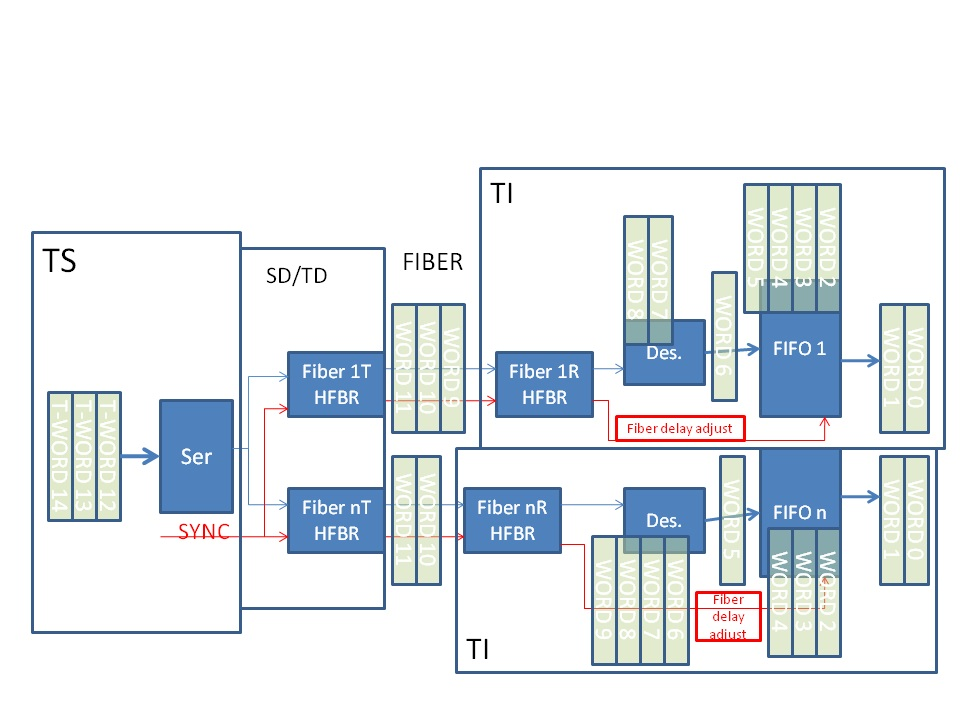
\includegraphics[width=1.0\columnwidth,keepaspectratio]{img/TrgSync.jpg}
	\caption{Trigger synchronization between TIs}
	\label{fig:TIsync}
\end{figure}

On the TI board, the deserialized trigger word is clocked into and clocked out of a FIFO using the 62.5MHz clock.  At the start-up, the FIFO is reset (0 words) and the FIFO read/write is disabled.  The serial trigger link is idle words only.  On trigger start, the TS starts trigger word transmission.  The TI will write the deserialized data (valid data, that is non-idle data word) to the FIFO.  After some pre-set delay (VME register controlled), the TS issues a ‘Trigger Start’ command on the SYNC link.  When TI receives the ‘Trigger Start’, the TI resets the trigger FIFO readout address, and enables continuous readout of the FIFO.  As the SYNC lines are fibre length adjusted and the 62.5MHz clocks are phase aligned, the trigger words from the TI board FIFO are synchronized across the system.
The trigger word also has the fine trigger timing information.  By decoding that, the TI board distributes the trigger in 4 ns precision, although the trigger word is serialized every 16 ns.  If the system clock phase is not adjusted, there will be a maximum of 4 ns skew among the clocks on the TI boards, so does the readout trigger.  The clock phase can be adjusted by SD if the skew is critical to the system.

D.	DAQ synchronization (trigger throttling) control
Because of the finite memory size and the randomness of the triggers, it is possible that the memory get overwhelmed somewhere in the system, which could cause problems in the DAQ system.   The TCS throttling mechanism is used to prevent the possible memory overflows, and to keep the DAQ synchronized.  Fig.~\ref{fig:DAQ_synchronization} shows the DAQ synchronization logic implementation.  Three methods are used to keep the DAQ synchronized.  They are Trigger rules and event limit setting, Pipeline DAQ, and Synchronization events (special events).

\begin{figure}[hbt]
	\centering
	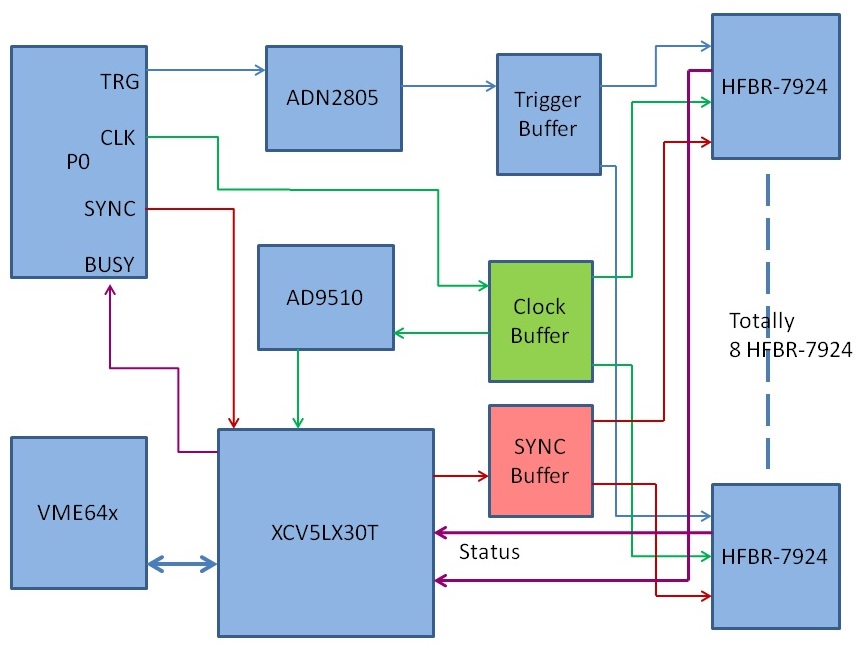
\includegraphics[width=1.0\columnwidth,keepaspectratio]{img/TDdiagram.jpg}
	\caption{DAQ synchronization}
	\label{fig:DAQ_synchronization}
\end{figure}


%REFERENCES
%[1] 	J. Gu etal. (2014, May). The TRIGGER/CLOCK/SYNC Distribution for TJNAF 12 GeV Upgrade Experiments    %https://coda.jlab.org/wiki/index.php/Trigger_distribution_overview
% [2] 	J. Gu. Description and technical information for the Trigger Supervisor (TS) module.  TJNAF, VA, 2013.  %Available: https://coda.jlab.org/drupal/system/files/pdfs/HardwareManual/TS/TS.pdf 
%[3] J. Gu, etal, 	“Design of the Trigger Interface and Distribution Board for TJNAF 12 GeV Upgrade,” IEEE Trans. Nucl. %Sci., Vol. 60, no. 5, pp 3714-3719, Oct. 2013

	
\subsection{Signal Distribution module (SD)(Cody)}

The Signal Distribution Board (SD) Fig.~\ref{fig:SDpic} module occupies the “B” switch card slot as specified in VITA 41. The main purpose of this module is to distribute signals received from payload slot 18 (Trigger Interface board) of a VXS crate to 16 other payload slots (ADC boards).

The Signal Distribution (SD) module distributes the 4 differential pair LVPECL signals from payload slot 18 to 16 VXS payload slots within the crate. This is done using the high speed point to point connections from the switch slot to each payload slot. The four signals distributed are length matched to minimize output jitter seen on all the payload slots. Three of the four remaining pairs are LVDS signals routed from the each payload module to the FPGA on the SD module. The last pair is an LVDS signal routed from the FPGA on the SD module to each payload module. Each of the 16 payload modules has a single-ended signal to the SD module and one from the SD module back to the payload module.

\begin{figure}[hbt]
	\centering
	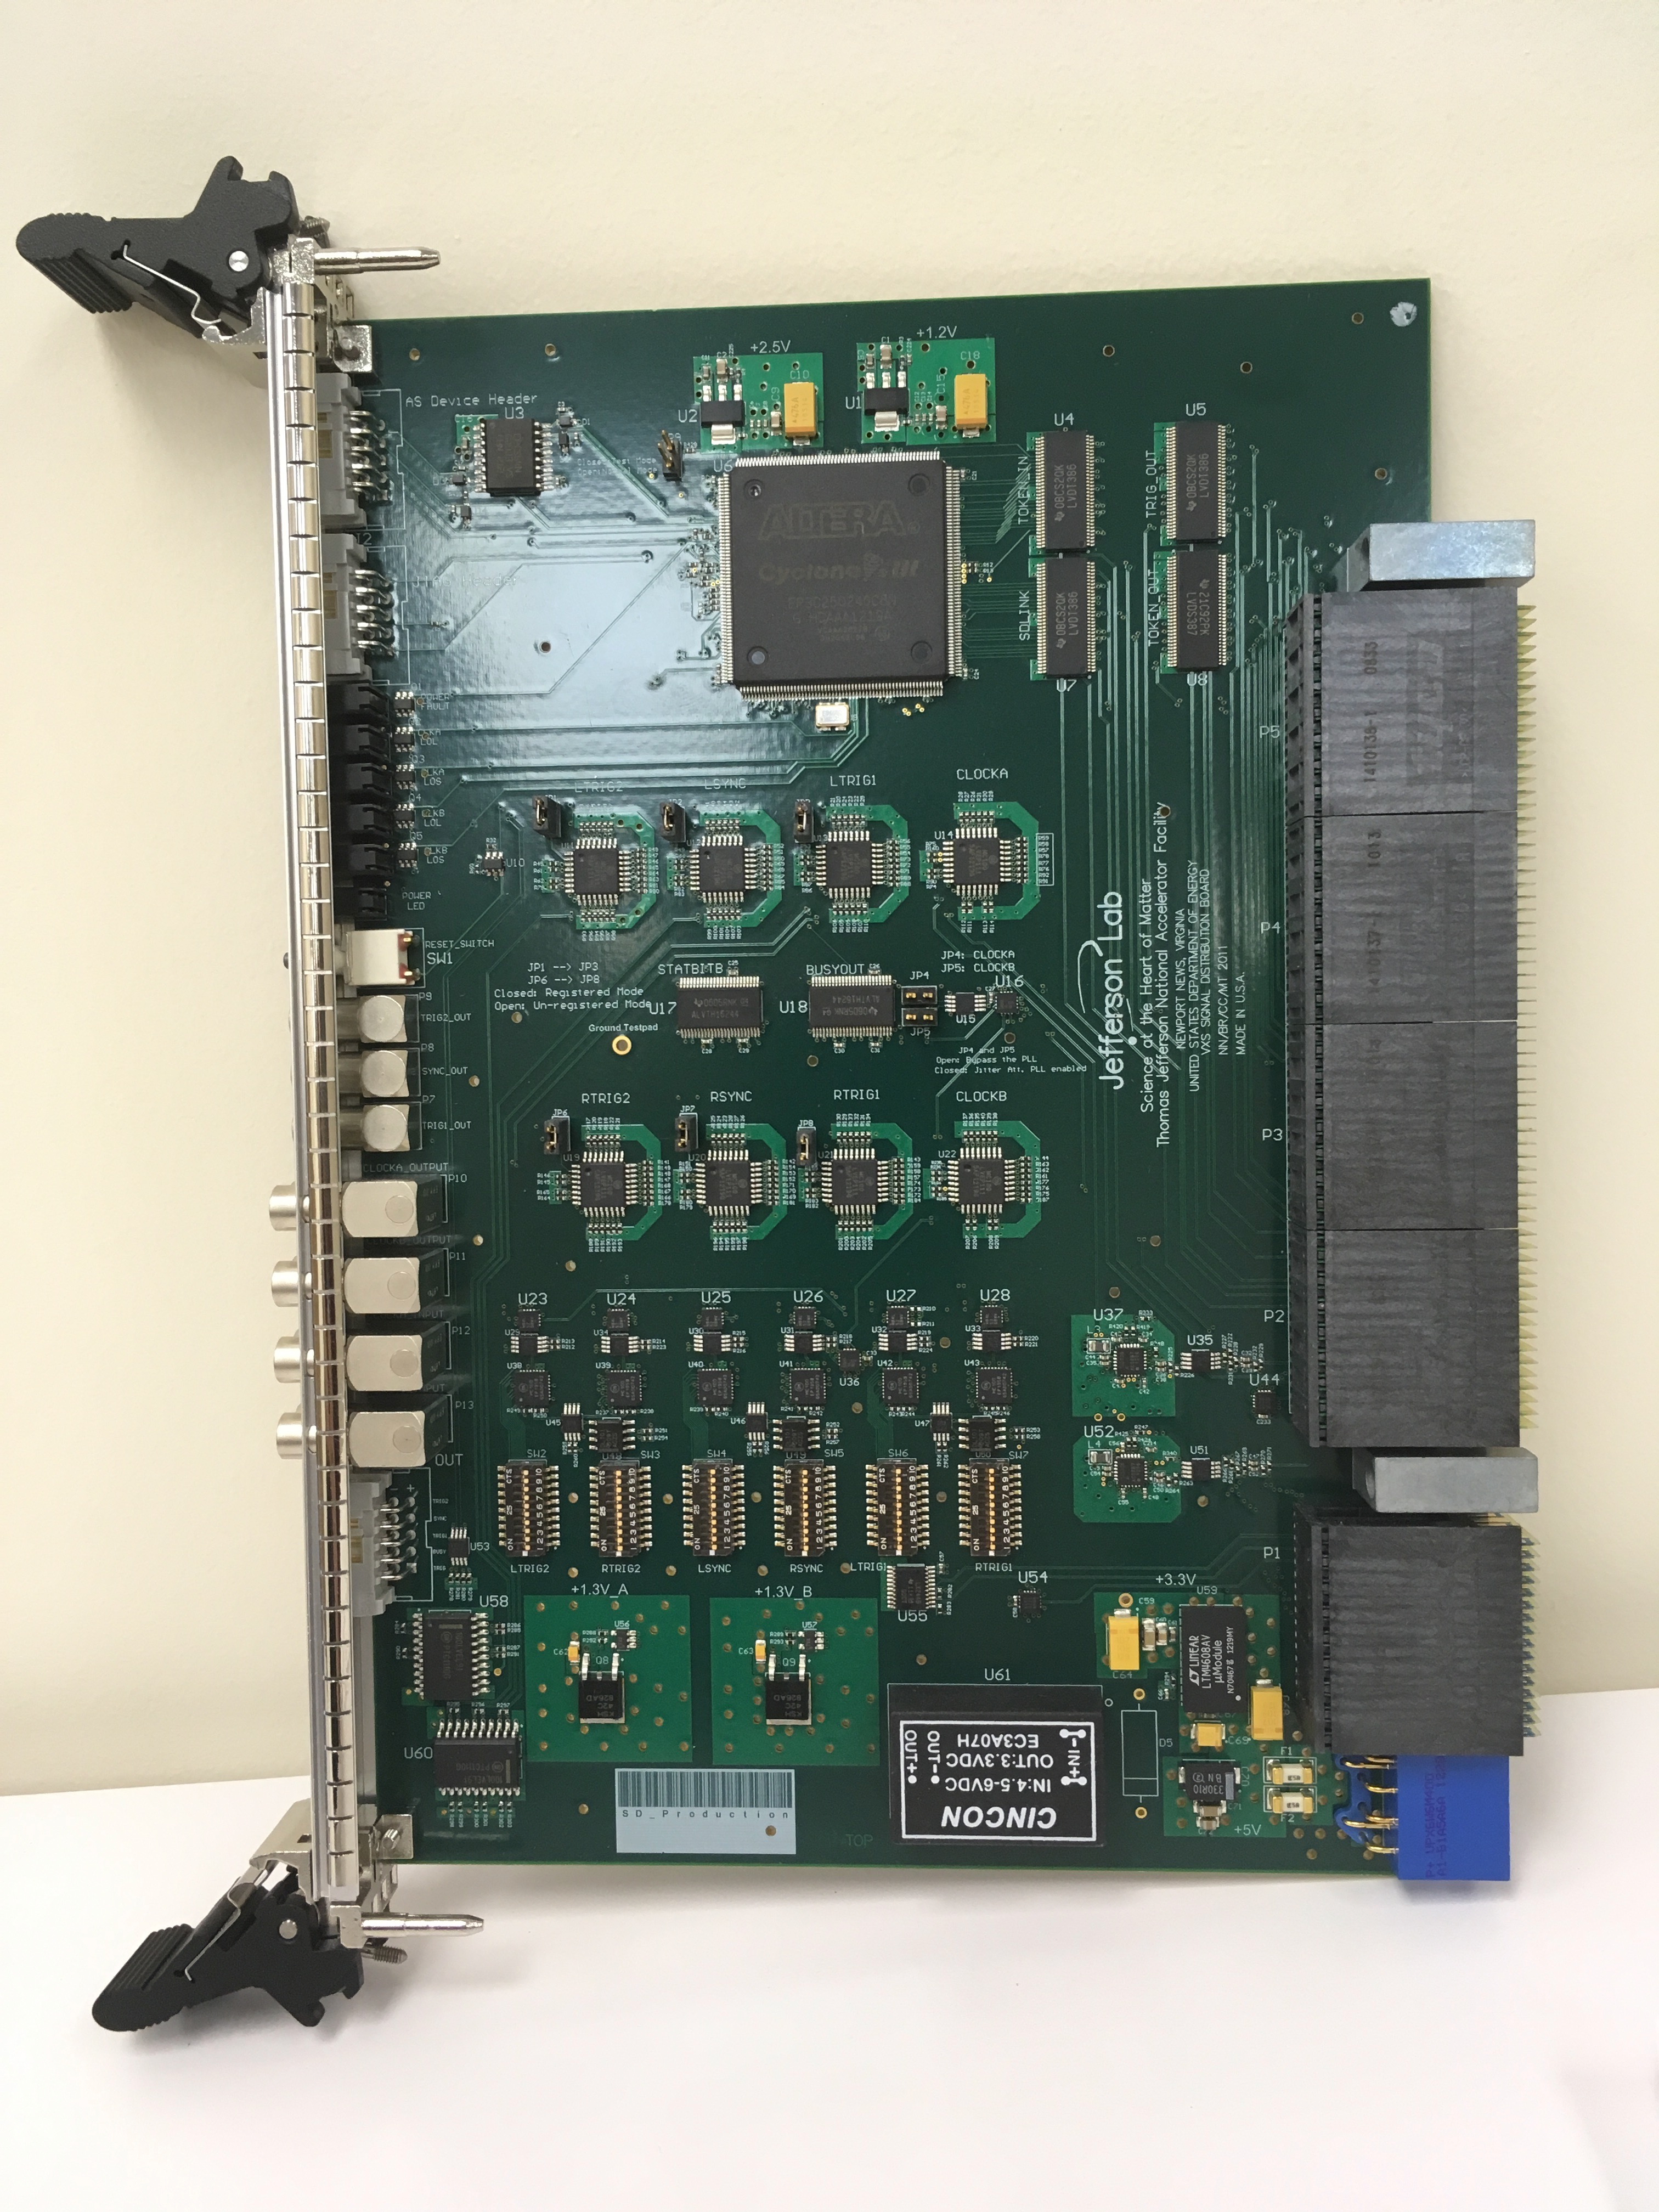
\includegraphics[width=1.0\columnwidth,keepaspectratio]{img/sd_board.jpg}
	\caption{Signal Distribution module (SD)}
	\label{fig:SDpic}
\end{figure}


\subsection{Flash ADC module (FADC250)(Hai)}

A 16-channel 250 MSPS pipelined flash ADC Fig.~\ref{fig:FADC250pic} with 12-bit precision was designed to digitize and process detector pulses for experiments at Jefferson Lab.  The FADC250 module Fig.~\ref{fig:FADC250_board} conforms to the VITA-41 VME64x switched serial (VXS) standard.  Each channel of the module accepts input signals on a LEMO style coaxial connector and has three user-selectable ranges (0.5 V, 1.0 V, 2.0 V).  Differential signal conditioning scales the input signals to within the dynamic range of the ADC and a single-pole low pass filter limits the signal bandwidth to the Nyquist band of the converter (125 MHz). Individual channel offsets are accomplished by means of DACs under VME control.  Each channel has its own dedicated ADC chip (Analog Devices AD9230). Both positive and negative polarity input signals are supported. The 250 MHz clock is distributed to the ADC chips through a low jitter (< 2 ps) network.  

\begin{figure}[hbt]
	\centering
	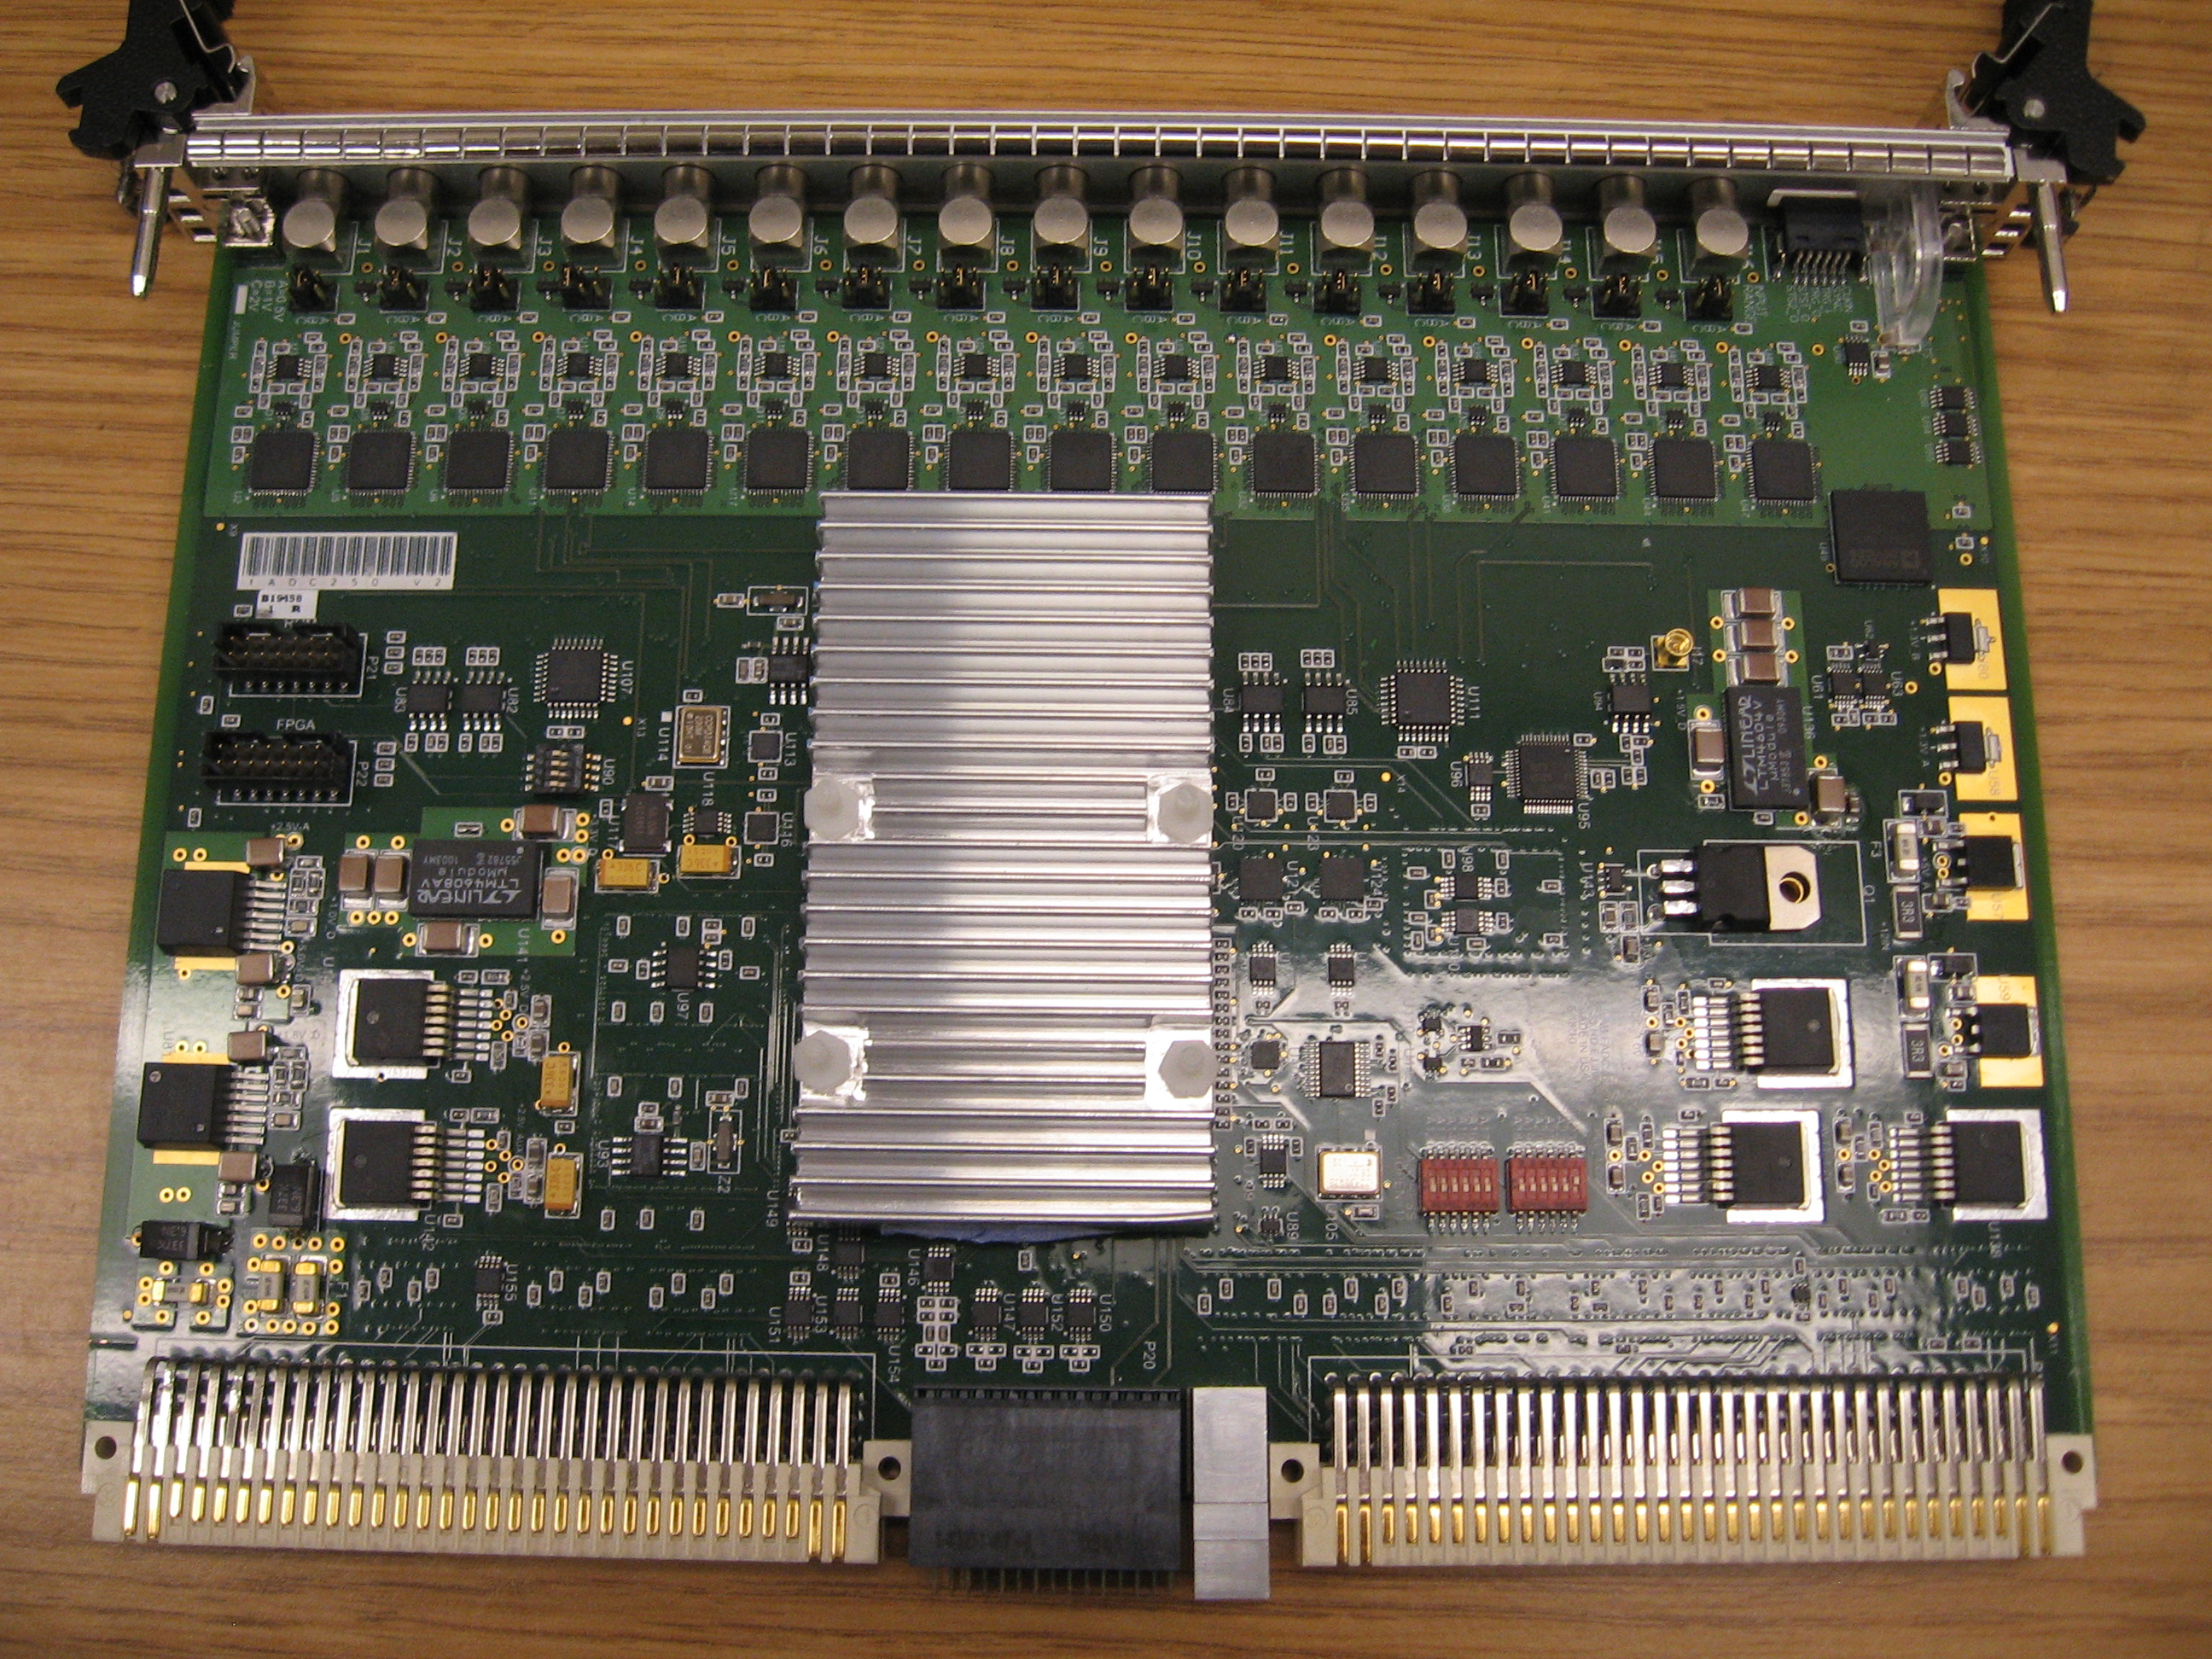
\includegraphics[width=1.0\columnwidth,keepaspectratio]{img/FADC250pic.jpg}
	\caption{Flash ADC module (FADC250)}
	\label{fig:FADC250pic}
\end{figure}

\begin{figure}[hbt]
	\centering
	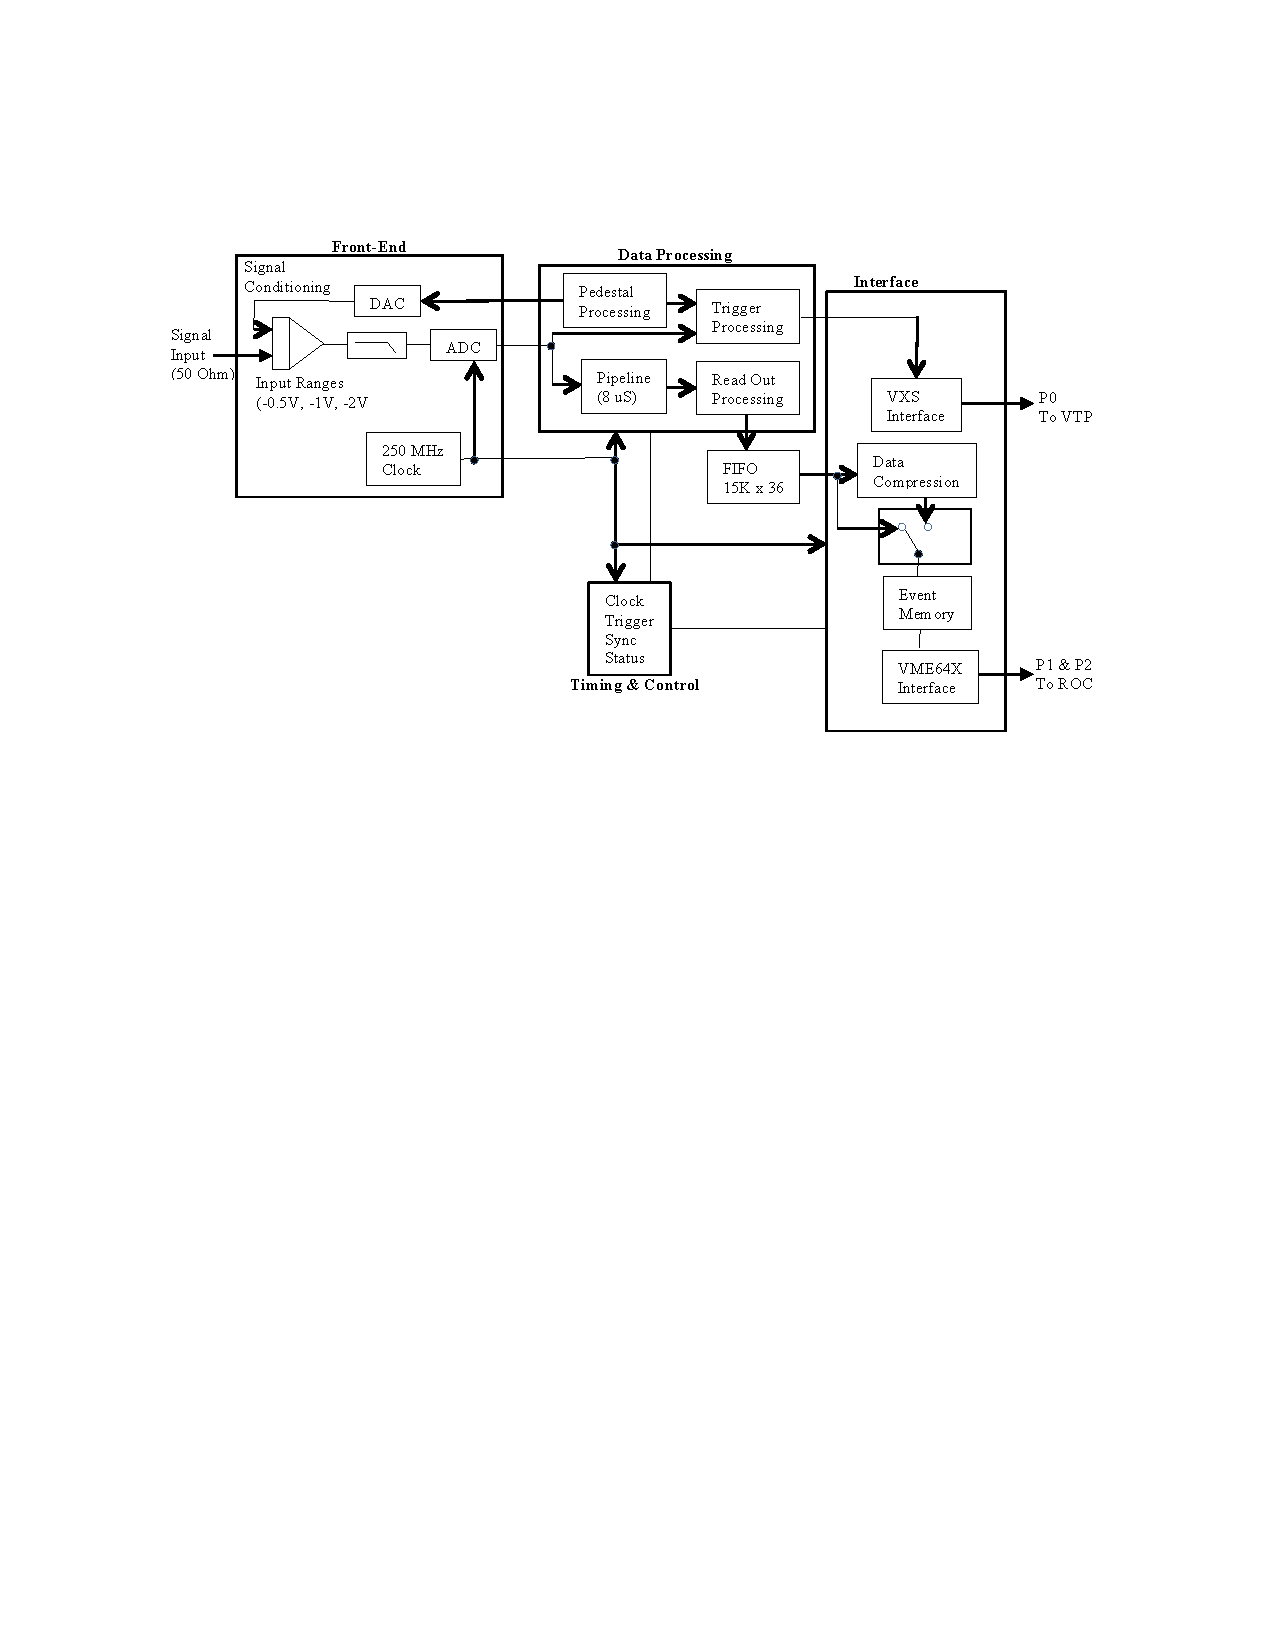
\includegraphics[width=1.0\columnwidth,keepaspectratio]{img/FADC250_Diagram.pdf}
	\caption{Flash ADC module diagram (FADC250)}
	\label{fig:FADC250_board}
\end{figure}

Digitized data from the 16 flash ADC chips is processed and formatted for readout in a pair of high performance Xilinx FPGAs. The digitized data from the ADCs follows two distinct paths.  Logic in the trigger data path pre-processes data for the trigger algorithms of the VXS Trigger Processor (VTP). The FADC250 module continuously streams this data to the crate’s VTP located in VXS switch slot A via high speed serial links of the VXS fabric.  Data from multiple VTPs and other modules are used to form a global trigger signal which is returned to the crates to initiate data readout.

The readout data path continuously stores digitized data for each channel in circular buffers. When a trigger signal is 
received by the module a programmable window up to 2 $\mu$s wide of digitized data is extracted from the buffers for
processing. The starting point of this window can be programmed up to 8 $\mu$s earlier than the arrival of the trigger
signal to account for the time required to form the trigger signal.  Zero suppression on the extracted data may be 
implemented for each channel using programmable thresholds.  A lossless data compression algorithm can also be applied to the data of each channel with typical compression factors of 2 to 3. The design is pipelined so that data from multiple triggers can be processed simultaneously.  Triggers separated in time by as little as 50 ns can be accepted by the module. The trigger number and trigger time (clock periods since last synchronization) are reported along with the channel data so that data from multiple modules can be correctly assembled into events. 

Data associated with a programmable number N of triggers is packaged into a block of data for read out over VME.  N can take values from 1 to 255, with 40 being a typical value chosen.  Data is stored in an on board 8 MB SRAM as 64-bit words to match the 64-bit high-speed (200 MB/s) dual edge VME Source Synchronous Transfer (2eSST) mode employed to read out the module.  

In order to save the overhead of setting up a DMA transfer for each FADC250 module in the crate a chained block readout mechanism with token passing is used.  A common address range is enabled for all modules in the crate but only the module having the token will respond to a read request.  A single logical DMA read is initiated by the VME crate controller and the first module in the chain supplies data from its block of event fragments.  When the first module’s block data is exhausted a token signal is passed to the next module in the chain and this module then proceeds to transmit its data from its block.  When that module’s data for the block is exhausted it transfers the token to the next module.  This continues until the data from the last module in the chain is exhausted.  Instead of passing the token the last module asserts the VME bus error signal (BERR) which terminates the DMA cycle.  The user returns the token to the first module and the process can begin again when the next block of events is ready for readout.  The user does not have to query the modules in advance to discover the number of words to read out.  The DMA is set up with a total number of words larger than any expected value for the entire crate.  Data from each module is tagged with the slot number to identify its source.  The token passes along a VXS signal line to VXS switch slot B where a module there (SD) routes it to the next enabled module.


\subsection{Discriminator Scaler module (DSC2)}

The Discriminator Scaler module (DSC2) Fig.~\ref{fig:dsc2_board} is a 16 channel general purpose discriminator and scaler module designed as a 6U VME card. It replaces an older design,improving on jitter, noise, crosstalk, and adding new features.

\begin{figure}[hbt]
	\centering
	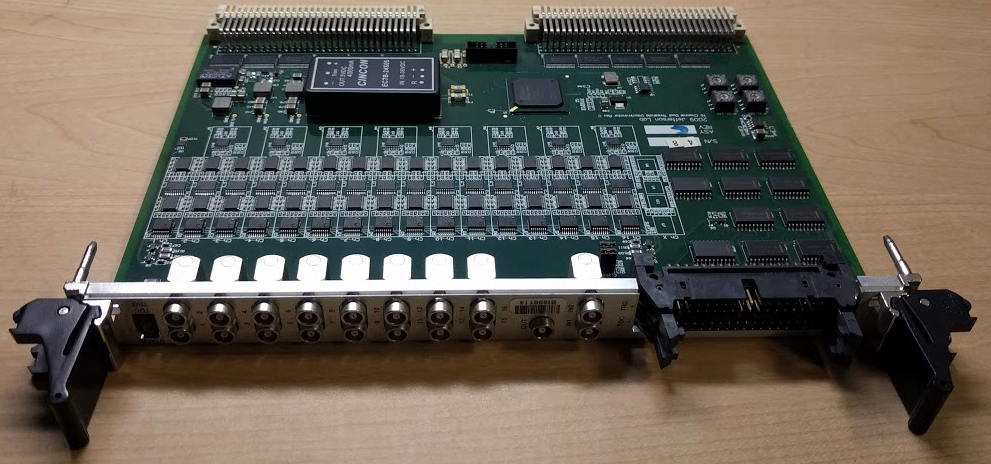
\includegraphics[width=1.0\columnwidth,keepaspectratio]{img/dsc2_board.png}
	\caption{Discriminator Scaler module (DSC2)}
	\label{fig:dsc2_board}
\end{figure}

\begin{center}
	DSC2 Specifications\\
	\begin{tabular}{| l | l |}
		\hline \hline
		Property			& Value				\\
		\hline
		{\bf Analog Discriminator}	&				\\
		Threshold			& 0 to -1023mV			\\
		Pulse width			& 4ns to 40ns			\\
		Dead-time			& 4ns typ. w/8ns pulser width	\\
		Maximum input rate		& $>$125MHz 			\\
		Ch-ch isolation			& $>$65dB			\\
		Threshold noise			& 1.3mV RMS typ.		\\
		Slew-rate delay disperson	& $<$20ps			\\
		Input-to-output delay		& $<$5ns			\\
		{\bf Digital Processing}	&				\\
		Digital delay step		& 4ns				\\
		Digital delay maximum		& 1us				\\
		Digital width maximum		& 1us				\\
		Maximum count rate		& 125MHz			\\
		\hline \hline
	\end{tabular}
\end{center}

\paragraph{Discriminator}
Inputs are single-ended LEMO and leading-edge discrimated by two different thresholds. Typically one threshold is used for time-to-digital applications and the other threshold is used for trigger applications. There are separate differential ECL outputs for each channel and threshold. Low jitter performance was an important goal of the design as this module will be used in high resolution applications. Fig.~\ref{fig:dsc2_jitter} shows the typical jitter as a function of a variety of input slew rate signals and threshold overdrive conditions.

\begin{figure}[hbt]
	\centering
	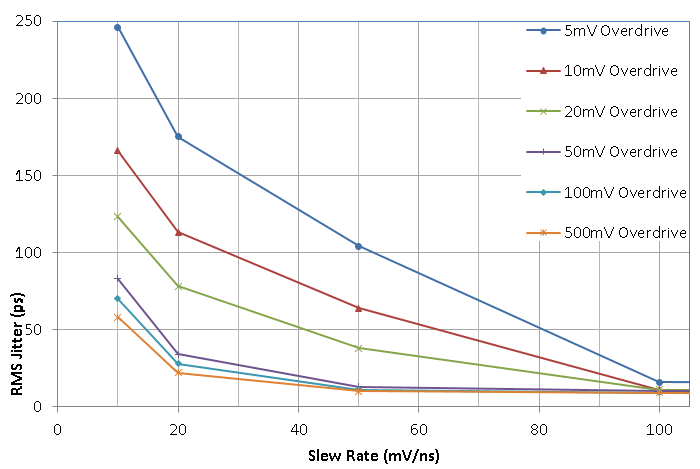
\includegraphics[width=1.0\columnwidth,keepaspectratio]{img/dsc2_jitter.png}
	\caption{Output Jitter vs Input slew rate and overdrive}
	\label{fig:dsc2_jitter}
\end{figure}

\paragraph{Digital Processing}
A Xilinx Spartan 3A FPGA is used to implement the VME interface, scalers, discriminator controls, and scaler event building features. Each channel and threshold has two scalers associated with it. The first scaler counts all threshold crossings for the input. The second scaler is gated using a front-panel input source, which can be useful to computing dead-time of channels and many other applications. Additionally, reference scalers are accumulated (a gated and ungated version) that count the elapsed time which can be used to normalize inputs scalers to Hz. All together there are 68 scalers, which can be slow to read over VME if using single-cycle transfers. An event builder is implemented that can synchronously read (and optionally clear) all scalers and build an event with this data. Over 100 events can be buffered and readout using the VME 2eSST protocol at 200MB/s.


\subsection{TDC modiles (v1190/v1290)(Sergey)}

Commercial CAEN V1190/V1290/V1290N TDC boards are used for timing measurements in PMT-based CLAS12 detectors (Fig.~\ref{fig:v1190_board}). V1190 has timing resolution about 100ps and V1290 about 35ps. All boards installed in CLAS12 DAQ are running on external 250/6=41.666 MHz clock rather then internal 40MHz clock. Different clock required compensation table remeasuring and reloading which was successfully complete.

\begin{figure}[hbt]
	\centering
	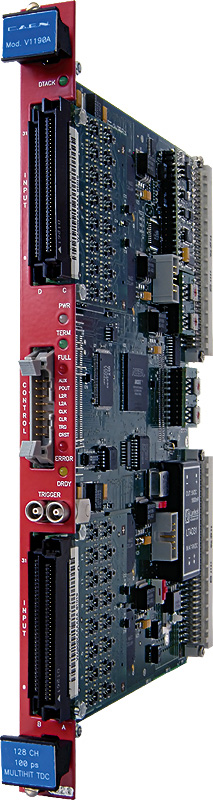
\includegraphics[width=0.2\columnwidth,keepaspectratio]{img/v1190_board.jpg}
	\caption{CAEN V1190 TDC module (V1190)}
	\label{fig:v1190_board}
\end{figure}

\subsection{Drift Chamber Readout Board (DCRB)}

\begin{figure}[hbt]
	\centering
	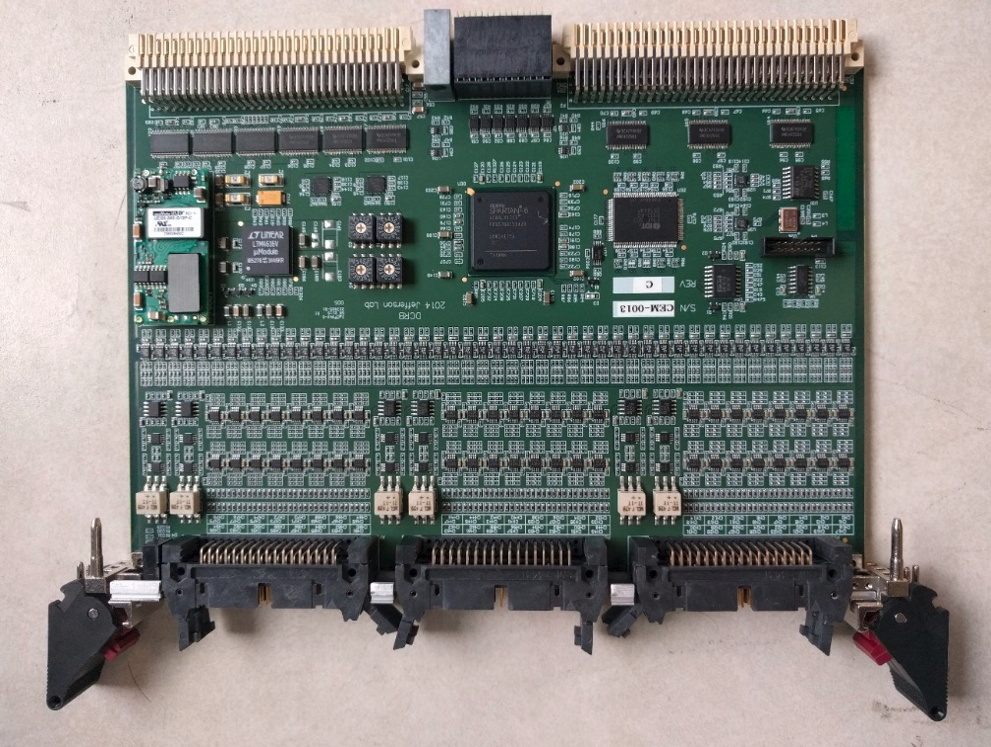
\includegraphics[width=1.0\columnwidth,keepaspectratio]{img/dcrb_board.png}
	\caption{Drift Chamber Readout Board (DCRB)}
	\label{fig:dcrb_board}
\end{figure}

The Drift Chamber Readout Board (DCRB) Fig.~\ref{fig:dcrb_board} is a 96 channel amplifier, discriminator, time-to-digital converter VXS module used to digitize and readout hits from the CLAS12 Drift Chambers. A single VXS crate of DCRB modules can readout a full region of the drift chambers for a single sector resulting in 18 VXS crates of DCRBs to instrument 6 sectors each having 3 regions of drift chamber.

\paragraph{Analog Inputs}
Each DCRB receives 96 differential analog signal pairs using twisted pair cabling from the drift chamber pre-amplifiers. The pre-amplfiers are located on the detector providing a gain of ~2.3mV/$\mu$A. On the DCRB each analog input channel is amplified by a voltage gain of 30 and then discriminated by a programmable threshold (common to all channels on the board with an effective chamber wire threshold range of 0 to 3.5/$\mu$A).

\paragraph{TDC Event Builder}
All discriminated channels go to a Xilinx Spartan 6 FPGA where a 96 channel 1ns resolution time-to-digital converter (TDC) is implemented in firmware. The TDC is based on the ISERDES2 shift register FPGA primitive that directly sample of the digital input with a single-data-rate (SDR) input register clocked at 1GHz. The TDC sampling clock is synchronized to the CLAS12 master oscillator making it easy to relate hit times in the drift chamber other detectors in CLAS12. TDC inputs are buffered supporting multiple hits allowing for an average hit rate of 4MHz per input before loss of data, which exceed the hits rates the chamber is designed for by a few orders of magnitude. Hits from groups of 16 channels are written into a large buffer that a linked-list content addressable memory (CAM) tracks for 16$\mu$s. When a L1A trigger signal is received a time window of hits is extracted from the TDC hit buffer. The readout time window times are supplied to the CAM, and the CAM provides the address of the last hit matching each readout time bin. The hit buffer is then read to extract the hit and also the address of the next hit in the buffer matching the time bin (this is the linked list behavior). The result is an extremely fast event builder with natural zero suppression that doesn't require time sorted data. Cleanup is accomplished by a timer that invalidates CAM entries after time bins are 16$\mu$s old. Hits for an event are assembled and buffered in a 2MByte external RAM which is readout through the VME bus using the 2eSST protocol at 200MB/s.

\paragraph{Calibration Support}
A programmable amplitude pulse generator is implemented that can inject test pulses directly to the DCRB differential amplifier inputs as well as to the pre-amplfiers that are on the detector. This provides a way to test points of failure, check channel gain, and check channel delays without any extra equipment. A scaler is implemented on each channel for slow control monitoring of all chamber wires.

\subsection{VXS Silicon Readout Module (VSCM)}
The CLAS12 Silicon Vertex Tracker (SVT) detector front-end utilizes the data driven FSSR2 ASIC for digitization. The VXS Silicon Readout Module (VSCM) Fig.~\ref{fig:vscm_board} was designed to interface the FSSR2 based front-end to the CLAS12 DAQ system. This system is capable of reading out all 33,792 SVT channels in 3 VXS crates.

\begin{figure}[hbt]
	\centering
	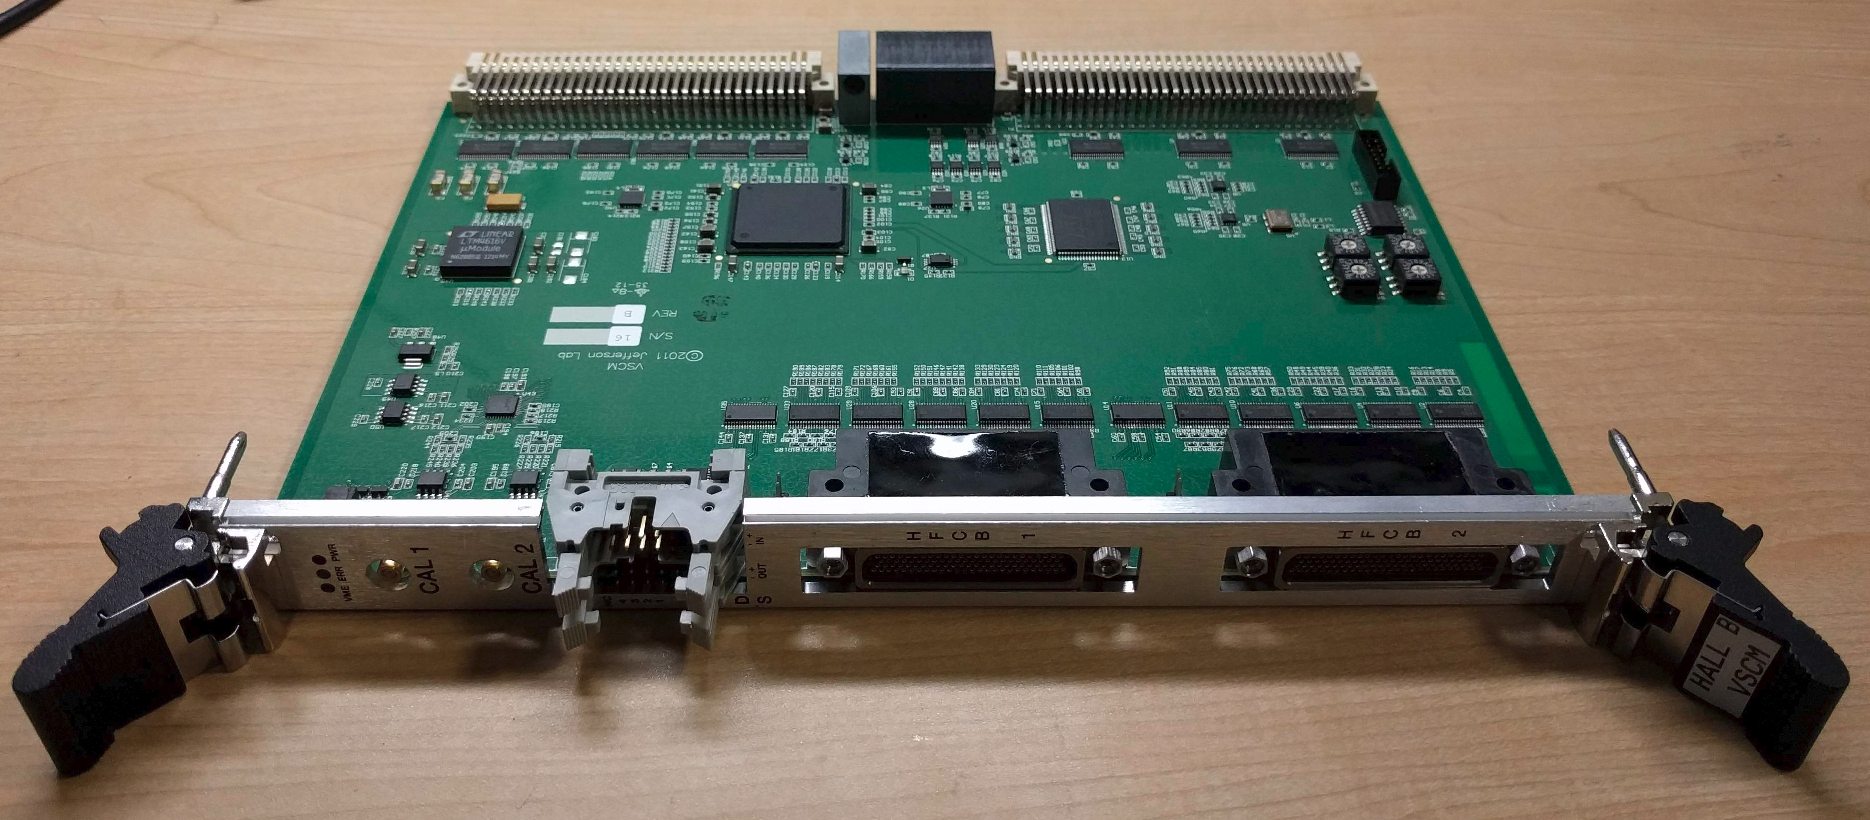
\includegraphics[width=1.0\columnwidth,keepaspectratio]{img/vscm_board.png}
	\caption{VXS Silicon Readout Module (VSCM)}
	\label{fig:vscm_board}
\end{figure}

The main features of the VSCM include:

\begin{itemize}
	\item Receives 8 FSSR2 streams, each at 840Mbps
	\item De-randomizes hits into an 8$\mu$s buffer
	\item 512k multi-hit, multi-event buffer
	\item Supports $>$1MHz trigger rate
	\item Programmable amplitude charge injector
	\item 1ns resolution time-to-digital converter (TDC)
	\item Per channel hit scaler
	\item FSSR2 synchronization, status, and control
\end{itemize}

\paragraph{Event Builder}
The VSCM deserializes the FSSR2 streams checking for errors and decoding the hits, which are stored in an 8$\mu$s circular memory. The hits are not guaranteed to be time ordered, so the timestamp and channel number are used to form the circular memory address (rather than storing in the order received). The VSCM also implements an 8 channel 1ns time-to-digital converter (TDC) which measures the logic OR of hits from each FSSR2 ASIC. This high time resolution is significantly better than the FSSR2 serial stream hit time resolution and is required for improved out-of-time hit rejection. The L1A trigger signal time is used to look back a fixed amount of time and extract a time window of hits from the circular memory, which correspond to the physics event. Non-zero hits are as assembled as an event and buffered in a 2MByte external RAM which is readout through the VME bus using the 2eSST protocol at 200MB/s.

The event data contains primarily two hit word types that together provide high time resolution and spatial hit resolution while keeping the front-end complexity low.

\begin{center}
	Low time resolution hit word\\
	\begin{tabular}{| l | l |}
		\hline \hline
		Property	& Description		\\
		\hline
		Hit Time	& 128ns resolution	\\
		Channel		& 0-1023 strip Id	\\
		Charge		& 0-7 threshold		\\
		\hline \hline
	\end{tabular}
\end{center}

\begin{center}
	High time resolution hit word\\
	\begin{tabular}{| l | l |}
		\hline \hline
		Property	& Description		\\
		\hline
		Hit Time	& 1ns resolution	\\
		Channel		& 0-7 chip Id		\\
		\hline \hline
	\end{tabular}
\end{center}

Fig.~\ref{fig:vscm_blockdiagram} shows the hardware block diagram of the module. Essentially a single low-cost Xilinx Spartan 6 FPGA was to implement the deserialization, buffering, event-building, monitoring, front-end configuration, time-to-digital conversion and monitoring.

\begin{figure}[hbt]
	\centering
	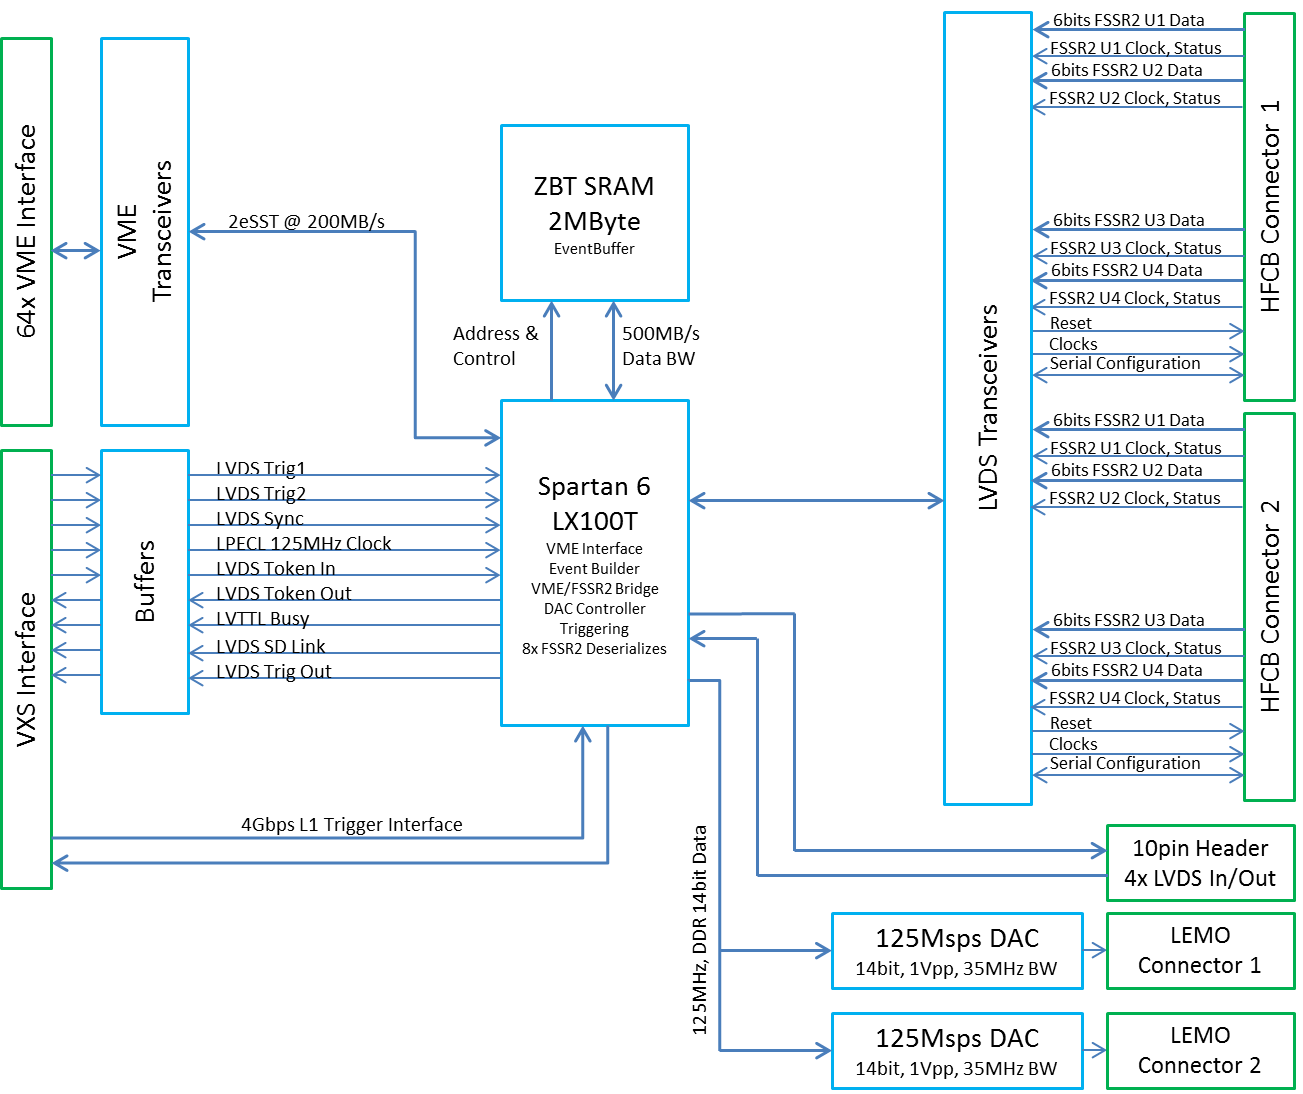
\includegraphics[width=1.0\columnwidth,keepaspectratio]{img/vscm_blockdiagram.png}
	\caption{VSCM Hardware Diagram}
	\label{fig:vscm_blockdiagram}
\end{figure}


\subsection{SSP board as fiber readout module(Ben)}

SSP (SubSystem Processor) was originally designed to work as part of CLAS12 trigger system. It is used to readout some front end electronics in DAQ system as well. Board description can be found in {ref CLAS12 Trigger}.